\begin{frame}
    \frametitle{Magnetómetro}
    \begin{center}
        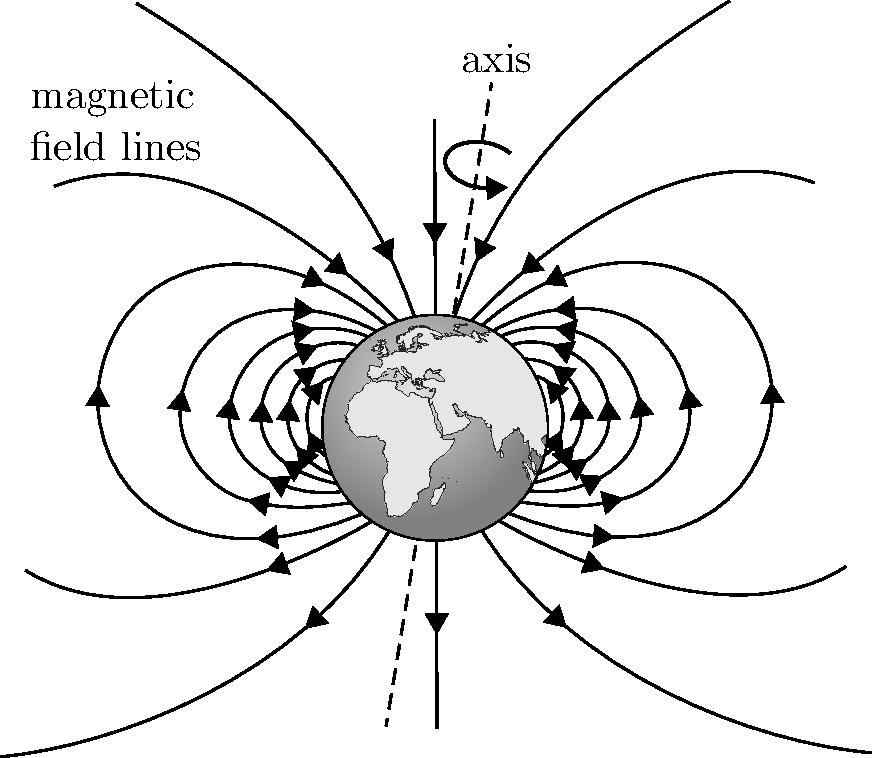
\includegraphics[width=0.2\columnwidth]{images/earth_magnetic_field.pdf}
        \hspace{1cm}
        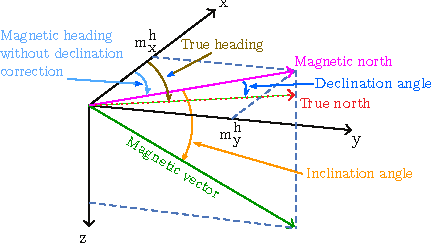
\includegraphics[width=0.3\columnwidth]{images/magnetic_field.pdf}
    \end{center}
    \scriptsize
    \begin{block}{Principio de funcionamiento}
        \begin{itemize}
            
            \item La Tierra es un imán masivo pero débil. Los polos del campo geomagnético son los polos magnéticos Norte y Sur. Los mismos se mueven constantemente y se encuentran a cierta distancia del eje de rotación de la Tierra.
    
            \item En cualquier punto del planeta, las líneas de flujo magnético pueden considerarse un vector $\vec{m}$ cuya magnitud y dirección pueden predecirse y trazarse con precisión.
            
            \item Describimos la dirección del vector $\vec{m}$ en términos de dos ángulos: \textbf{ángulo de Declinación} ($D$) e \textbf{ángulo de Inclinación} ($I$).
            
            \begin{itemize}
                \scriptsize
                \item Una proyección horizontal del vector $\vec{m}$ apunta en la dirección del norte magnético y el \textbf{ángulo de declinación} $D$ se mide desde el norte verdadero, en el sentido de las agujas del reloj hasta esa proyección.
            
                \item El \textbf{ángulo de inclinación} $I$ del vector se mide en un plano vertical hacia abajo desde la horizontal hasta $\vec{m}$.
                
                \item La longitud del vector, la \textbf{intensidad del campo magnético}, se mide con un magnetómetro en unidades de Tesla (T) y para la Tierra varía de $25-\SI{65}{\micro\tesla}$.
            \end{itemize}
        \end{itemize}
    \end{block}
\end{frame}


\begin{frame}
    \frametitle{Compass}
    \scriptsize
    \begin{figure}[!h]
        \centering
        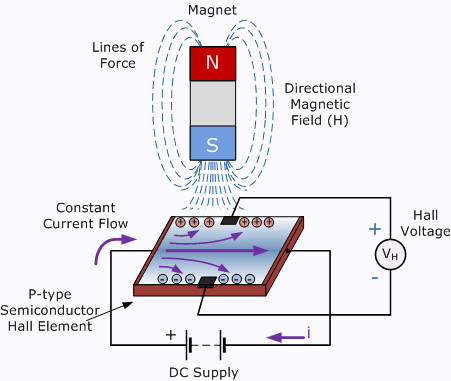
\includegraphics[width=0.3\columnwidth]{electromagnetism.jpg}
    \end{figure}

    \begin{block}{Principio de funcionamiento}
        \begin{itemize}
        \item El elemento clave de la mayoría de los magnetómetros modernos es un sensor de efecto Hall, un dispositivo semiconductor que produce un voltaje proporcional a la intensidad del campo magnético en una dirección normal al flujo de corriente.
        \item Normalmente, tres sensores de efecto Hall se empaquetan juntos y se disponen de modo que sus ejes sensibles sean ortogonales.
        \item Las tres salidas de dicho magnetómetro triaxial son los componentes del vector de intensidad del campo magnético de la Tierra m medido en la estructura del cuerpo $\bodyCoordSystem$.
        \end{itemize}
    \end{block}
\end{frame}

\begin{frame}
    \frametitle{Compass}
    \begin{figure}[!h]
        \centering
        \subfloat[Magnetic field intensity]
        {
            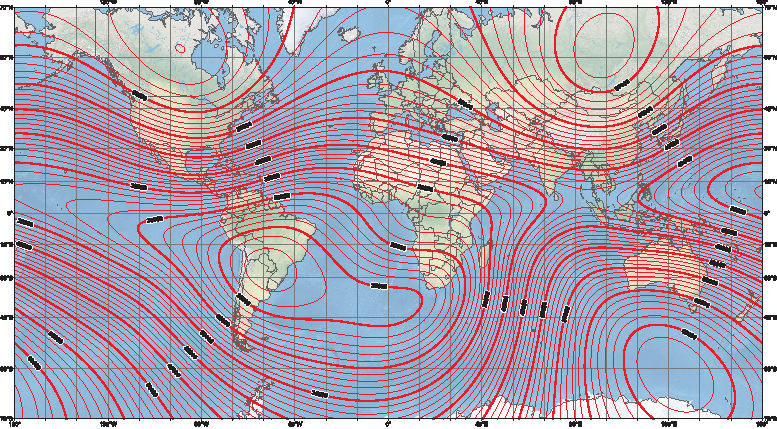
\includegraphics[width=0.3\columnwidth]{images/magnetic_field_intensity.pdf}
        }
        \subfloat[Magnetic declination]
        {
            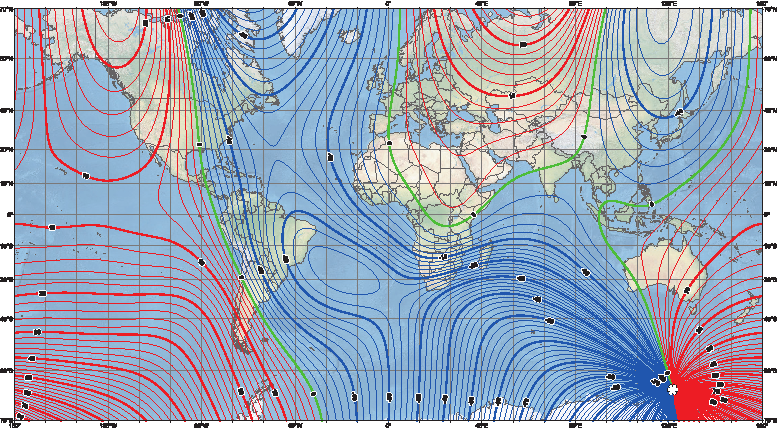
\includegraphics[width=0.3\columnwidth]{images/magnetic_declination.pdf}
        }\\
        \subfloat[Magnetic inclination]
        {
            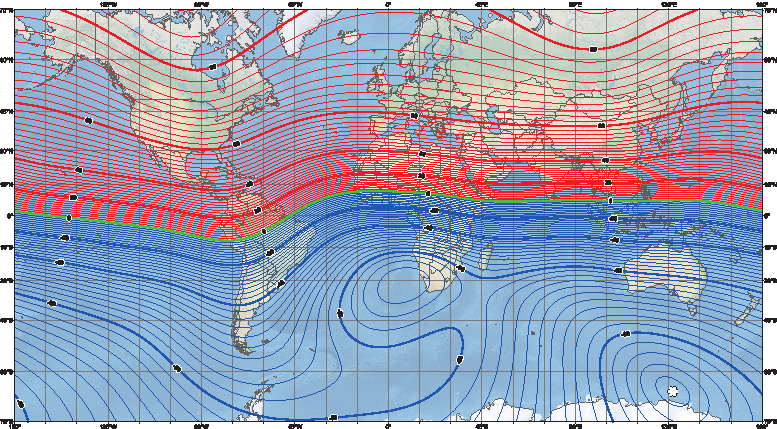
\includegraphics[width=0.3\columnwidth]{images/magnetic_inclination.pdf}
        }
    \end{figure}
\end{frame}


\begin{frame}
    \frametitle{Compass}

    \begin{center}
        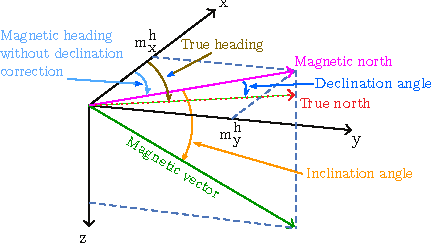
\includegraphics[width=0.5\columnwidth]{images/magnetic_field.pdf}
    \end{center}

    \begin{itemize}
        \item Exteroceptivo
        \item Pasivo
        \item Mediciones absolutas
        \item Muy ruidoso. Problemas con los componentes propios del los robots (componentes electromagnéticos) y con objetos del entorno materiales ferromagnéticos (estructuras metálicas)
    \end{itemize}
\end{frame}

\begin{frame}
    \frametitle{Compass}

    \begin{center}
        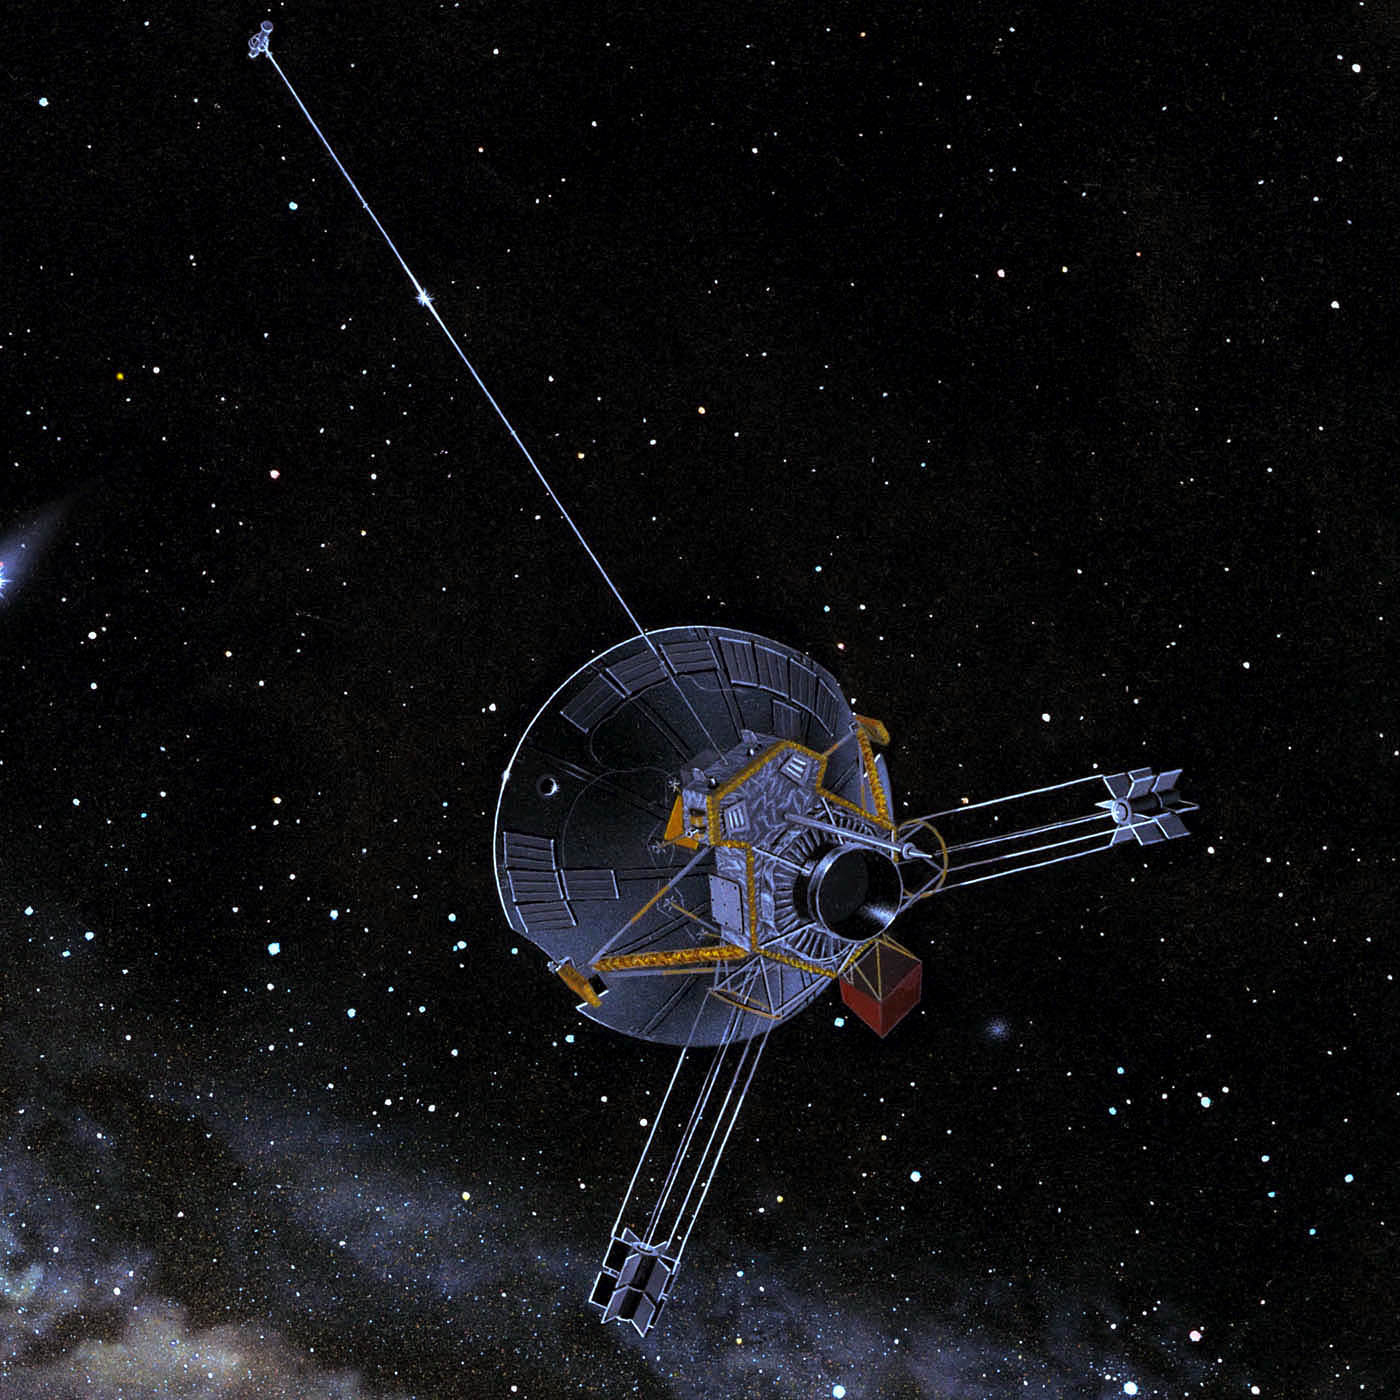
\includegraphics[width=0.5\columnwidth]{pioneer_10.jpg}
    \end{center}
\end{frame}


\begin{frame}
    \frametitle{Compass}
    \scriptsize
    Considere un marco de coordenadas inerciales $\{ 0 \}$ con su eje $z$ verticalmente hacia arriba y su eje $x$ apuntando hacia el norte magnético. Por lo tanto, el vector de intensidad del campo magnético $I$ se encuentra en el plano $xz$.

    \begin{equation*}
        \toCoord{\vec{m}}{0}
    \end{equation*}

    donde $B$ es la intensidad del campo magnético e $I$ el ángulo de inclinación. En un frame de cuerpo fijo $\{ B \}$ en una orientación arbitraria expresada en términos de ángulos de roll-pitch-yaw la intensidad del campo magnético es

    \begin{equation}
        \label{eq:compass}
        \toCoord{\vec{m}}{0} = \transform{0}{B}^{-1} \vec{m}
    \end{equation}
    donde
    \begin{equation*}
        \transform{0}{B} = R_{z}(\theta_{y}) R_{y}(\theta_{p}) R_{x}(\theta_{r})
    \end{equation*}

    \begin{equation*}
    \toCoord{\vec{m}}{0} =
    \begin{bmatrix}
        m_{x} \\
        m_{y} \\
        m_{z}
    \end{bmatrix}
    \end{equation*}

    Igualando esta ecuación con \ref{eq:compass} podemos despejar el ángulo yaw:

    \begin{equation*}
        \theta_{y} = \tan^{-1} \dfrac{\cos \theta_{p}  \left( m_{z} \sin \theta_{r} - m_{y} \cos \theta_{r} \right)} {m_{x} + B \sin I \sin \theta_{p}}
    \end{equation*}

    Definimos el ángulo yaw como la orientación del eje $x$ del marco $\{ B \}$ con respecto al norte magnético. Para obtener el ángulo de orientación con respecto al norte verdadero, restamos el ángulo de declinación local:

    \begin{equation*}
        \prescript{tn}{}{\theta_{y}} = \theta_{y} - D
    \end{equation*}

\end{frame}
